\chapter{Introducción}
\label{sec:intro} % etiqueta para poder referenciar luego en el texto con ~\ref{sec:intro}
\pagenumbering{arabic} % para empezar la numeración con números

En este capítulo se introduce el proyeto.

En un primer apartado se realiza una breve introducción al software libre, explicando
sus conceptos básicos, pero centrándonos sobre todo en la ingeniería
dedicada al estudio de este tipo de software. Se incluye, además, una mención a
otras herramientas que comparten el objetivo de analizar proyectos de software libre.
Asímismo, haremos una descripción de las fuentes de información de donde el proyecto
realizará la extracción de datos relevantes.

Por último, daremos a conocer las principales características del lenguaje de
programación en el que está escrito el código fuente y justificaremos su
adecuación a nuestros propósitos.



\section{Software libre}
\label{sec:software-libre}

Todo programa que sea considerado software libre debe ofrecer una serie de
libertades. Se resumen en:
libertad de usar el programa con cualquier fin,
sin necesidad de comunicarlo a los desarrolladores;
libertad de estudiar el código fuente del programa y modificarlo
adaptándolo a nuestras necesidades, sin necesidad de hacer públicas las
modificaciones;
libertad de distribuir copias, tanto binarios como código fuente,
modificadas o no, gratis o cobrando por su distribución;
libertad de modificar el programa y publicar las mejoras para beneficio
de la comunidad.


\subsection{Ingeniería del software libre}
\label{subsec:SLE}

El enfoque sistemático y cuantificable que propone la ingeniería del software
siempre tuvo como barreras las propias de las formas en que el software ha
sido desarrollado, publicado y distribuido. Aspectos como el formato binario,
oscurantismo en modelo de negocio y limitaciones comerciales han impedido
validar resultados por parte de equipos independientes.

El reciente auge del software libre aporta novedades a esta ingeniería del software.
La implantación de Internet junto con las licencias que fomentan la colaboración
en el desarrollo del software, han favorecido a que además del código fuente,
se diponga de repositorios de versiones donde observar la evolución del software
o listas de correo que reflejan las comunicaciones durante el desarrollo.
De estas fuentes puede obtenerse gran cantidad de datos de valor,
incluso de forma automatizada.

Varios factores son los aportados a la ingeniería del software tradicional
desde ingeniería del software libre:
\begin{itemize}
\item
Visión temporal incorporada al análisis: necesaria ya que el proceso de creación
cambia y su evolución analizada de forma continua proporciona información
muy interesante (lenguajes más usados, evolución de colaboradores de un proyecto)
destinada a servir de ayuda en la toma de decisiones.
\item
Análisis a gran escala: dada la inexistencia de impedimentos para ampliar
el análisis al conjunto global de los proyectos de software libre gracias a la
disponibilidad de la información generada durante su desarrollo.
La ingeniería del software libre hace posible evaluar un proyecto
dentro de entornos globales y de menor envergadura, ofreciendo información desde
distintos puntos de vista, lo cual beneficia en la mencionada toma de decisiones.
\end{itemize}

En cierto modo, la ingeniería del software libre plantea cuantificar unos
parámetros que nos permitan pronosticar con precisión costes, recursos y plazos.
En la actualidad el software libre carece de estos métodos, aunque la
disponibilidad del código fuente y la información generada durante su desarrollo
constituye un enorme potencial para que cambie esta situación.
La ingeniería del software pretende también aplicar las cualidades de la
ingeniería del software en el desarrollo de proyectos de software libre,
de modo que se garantice a los desarrolladores la forma de generar
software de calidad siguiendo los paradigmas adecuados.
La ingeniería del software pretende aportar resultados objetivos y contrastables
acerca de la evolución del software y desterrar así apreciaciones que algunos dan
por ciertas.
A corto plazo, la ingeniería del software libre tiene por objetivo realizar
un análisis completo del desarrollo del software libre permitiendo indagar
en los procesos
que están involucrados, así como una adaptación de modelos de previsión de
costes del estilo de COCOMO en el software propietario.
Puede considerarse que el software libre funciona gracias a una ``mano negra'',
que hace que el software se genere mágicamente. Es por ello que la ing del 
soft libre busca comprender los elementos e interacciones que engloba esta
laguna de conocimiento denominada``mano negra''.

Se hace imprescindible un análisis de los datos relacionados con el software
libre para poder alcanzar los objetivos, previamente descritos, que la
ingeniería del software libre se propone. Deberá procurarse que las herramientas
empleadas para ello estén disponibles para que grupos independientes puedan
verificar los resultados.
En este proceso de análisis pueden diferenciarse dos fases.
En la primera etapa, un grupo de utilidades independientes entre sí recogen
datos cuantificables del código fuente y otros flujos de información y
almacenan los resultados en un formato intermedio, que serán analizados en
la siguiente fase. Lo ideal es que esta fase se realice de forma automática.
La segunda fase, no tan madura como la anterior, integra programas que toman
como entrada los parámetros almacenados en el formato intermedio y se dedican
a su análisis, procesado e interpretación. Se han propuesto varios modos de
analizar los resultados, de entre las que destacamos:
herramientas de análisis de clústers, que a partir de porciones reducidas de
datos, agrupan los interrelacionados con el objetivo de categorizarlos;
herramientas de análisis estadístico, que simplifican el procesado de grandes
cantidades de datos y permiten mostrar gráficamente los resultados;
una interfaz web, cuyo fin es, además de proporcionar acceso a los
resultados de este gran proyecto, la aplicación de los programas que
generan este interfaz a otros proyectos de software libre, de modo que surja
una realimentación del proyecto global.
\\[0.5cm]
En cuanto a las fuentes a analizar, la que alberga mayor información
en potencia es el código fuente. De él pueden extraerse parámetros como tamaño,
número de líneas lógicas o físicas, número de desarrolladores, lenguaje de
programación, etc. Uno de los estudios pioneros en este campo se encarga de
calcular el número de líneas físicas de código de proyectos de software libre
y aplicar el modelo COCOMO para obtener conclusiones en torno al coste, tiempo
y recursos empleados en el desarrollo del software.

Otras fuentes de interés son aquellas donde se produce intercambio de
información entre desarrollCadores, como listas de correo o canales de IRC.
De estos últimos aún no se han definido claramente los parámetros a buscar,
mientras que de las listas interesa recuperar de cada mensaje del archivo:
el nombre y dirección del autor, la fecha, e incluso podría cuantificarse
la longitud del mensaje.

Existe otro tipo de fuentes de información compuesto por una serie de
herramientas que sincronizan el trabajo de los distintos desarrolladores
de un software. Las más comunes son los sistemas de control de versiones,
de los cuales obtener conclusiones acerca de la participación de cada
desarrollador; y los sistemas de gestión de errores.

Una modalidad más de recopilación, quizás aplicable en un futuro, es la
relacionada con la información personal de los desarrolladores,
que a día de hoy no suele facilitarse, y que ayudaría
a conocer con mayor profundidad la comunidad del software libre. Además, si
se dispusiera de los datos laborales de estos desarrolladores ---como proyectos
en los que colaboró y horas empleadas--- podría establecerse una previsión
de costes y recursos para futuros proyectos de software libre.


\subsection{Otras herramientas para el análisis de proyectos de software libre}
El presente proyecto se integra con los previamente desarrollados por el
proyecto Libre Software Engineering, perteneciente al GSyC~\cite{GSYC}
(Grupo de Sistemas y Comunicaciones) de la Universidad Rey Juan Carlos.
Sus trabajos se centran en la medición cuantitativa de las características
del software libre, con especial atención en las herramientas utilizadas en
su desarrollo, los agentes que en él intervienen y los métodos seguidos;
todo ello bajo una perspectiva ingenieril, y no tanto social o económica.

En la web del proyecto~\cite{LSE} se encuentran,
aparte de documentos relacionados con su actividad, una relación de las
herramientas usadas para recopilar la información sobre el proceso de desarrollo
de software libre, junto con los resultados obtenidos de su aplicación sobre
un conjunto representativo de proyectos de software libre.

Entre las utilidades empleadas se encuentran herramientas que extraen
y obtienen estadísticas a partir de logs de repositorios CVS y las exportan
a formato XML o a una base de datos~\cite{CVSWWW, CVS} (\textit{CVSAnalY});
recogen código de repositorios CVS y de paquetes deb y rpm, que es analizado
y exportado a XML o a base de datos~\cite{GlueWWW, Glue} (\textit{GlueTheos});
realizan un conteo de las líneas de código reales de un determinado software
\cite{Sloc} (\textit{SLOCCount});
o llevan a cabo un análisis estadístico acerca de la distribución de la
propiedad del código dentro de un paquete de software~\cite{Codd} (\textit{COOD}).



\section{Fuentes de información a estudio}
De entre las fuentes de donde recopilar los parámetros de interés acerca de
la creación de software libre, nos centraremos en las que constituyen un
mecanismo de intercomunicación y colaboración entre desarrolladores y usuarios.
Los foros web de SourceForge, el sistema de seguimiento de errores de Debian,
y las listas de correo de Mailman fueron los elegidos.


\subsection{Foros en SourceForge} \label{intro_foros}
SourceForge es uno de los principales sitios web de soporte al desarrollo
de proyectos, mayoritariamente de software libre. Supone una convergencia de
herramientas, en un principio sólo disponibles de manera individual y con la
necesidad de configuración para el trabajo en conjunto. Con la llegada de
SourceForge y servicios del estilo, el desarrollador se dedica en exclusiva
a su proyecto, desentendiéndose de la puesta en marcha y administración de la
infraestructura de colaboración. Conviene no confundir el sitio
(\url{http://sourceforge.net}) con el conjunto de programas que lo mantienen
en pie, que dejó de ser software libre a finales de 2001.

Los servicios destacables que proporciona SourceForge a un proyecto son:
\begin{itemize}
\item Hospedaje de las páginas web del proyecto, pudiendo ser dinámicas y
hacer uso de una base de datos.
\item Página con datos resumen sobre el estado del proyecto, estadísticas, etc.
\item Uso y gestión de tantos foros y listas de correo como el administrador
estime oportuno.
\item Servicio de CVS para desarrolladores y usuarios anónimos.
\item Granja de compilación con diferentes sistemas operativos y plataformas,
permitiendo generar software portable.
\item Servicio de subida y descarga de software, replicado en servidores de
todo el mundo.
\item Sistemas de seguimiento de informes de errores, tareas pendientes,
peticiones de soporte y mejora; que los administradores priorizan y asignan
a cada desarrollador.
\end{itemize}

Dentro de los servicios recién comentados figuran los foros web. Éstos son
un hervidero de consultas relativas a dificultades en el manejo del
software, de sugerencias sobre la incorporación de funcionalidades ausentes,
y peticiones de ayuda al resto de usuarios ante problemas particulares;
por lo que generan un considerable volumen de información referente a la
evolución de los proyectos merecedor de ser tenido en cuenta en un estudio
como el que se pretende realizar.

El análisis de los foros web de SourceForge presenta complicaciones ya que
ni tan siquiera se dispone de los scripts mediante los que se genera,
haciendo necesario el estudio de la estructura a través de la observación
del código fuente. Por tanto, existe la posibilidad de que esta estructura
sea modificada de pronto y deba rehacerse su estudio.

Respecto a su interfaz, estos foros proporcionan modos de presentación
variados:
\begin{itemize}
\item \textbf{Anidado} (\textit{Nested}). Cada página muestra una sucesión
de mensajes donde aquellos que responden a otros ---conformando un hilo---
se presentan anidados. Siguen una ordenación descendente por fecha de
modificación de los hilos.
\item \textbf{Plano} (\textit{Flat}). Cada página muestra una sucesión de
mensajes, ordenados de forma descendente por su fecha de envío.
\item \textbf{Por hilos} (\textit{Threaded}). Idéntico a modo anidado pero
mostrando hiperenlace a mensaje, junto con su autor y fecha, en lugar de cada
mensaje.
\item \textbf{Último} (\textit{Ultimate}). Cada página muestra una sucesión
de hiperenlaces a hilos, junto con el autor del mensaje inicial del hilo,
número de respuestas y la fecha del último mensaje enviado. Siguen una
ordenación descendente por fecha del último mensaje enviado.
\end{itemize}
Todos ellos permiten elegir la cantidad de elementos a mostrar por página.
De entre todos, el elegido del que extraer los datos de interés, de acuerdo
a los requisitos, será el modo de representación \textit{último}.

 \begin{figure}[H]
    \centering
    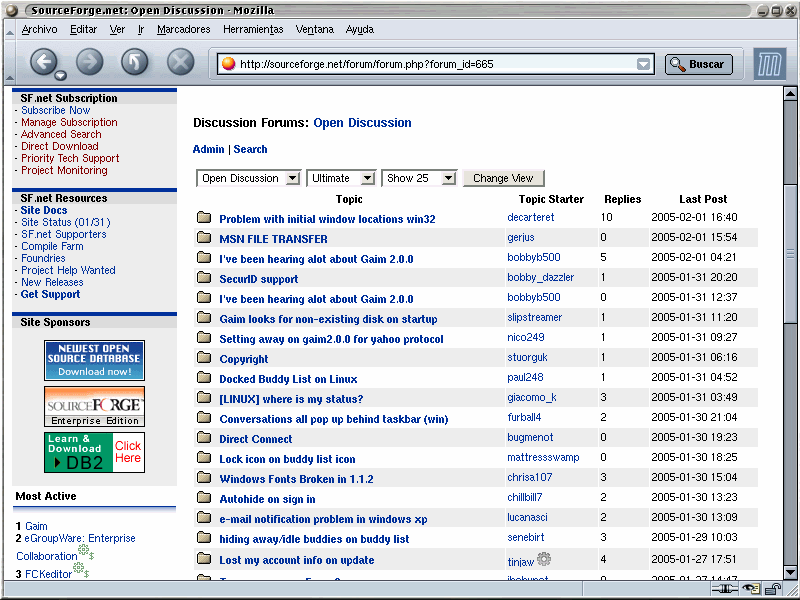
\includegraphics[bb=0 0 800 600, width=12cm, keepaspectratio]{img/foro1}
    \caption{Página con enlaces a hilos}
    \label{figura:foro_hilos}
 \end{figure}

 \begin{figure}[H]
    \centering
    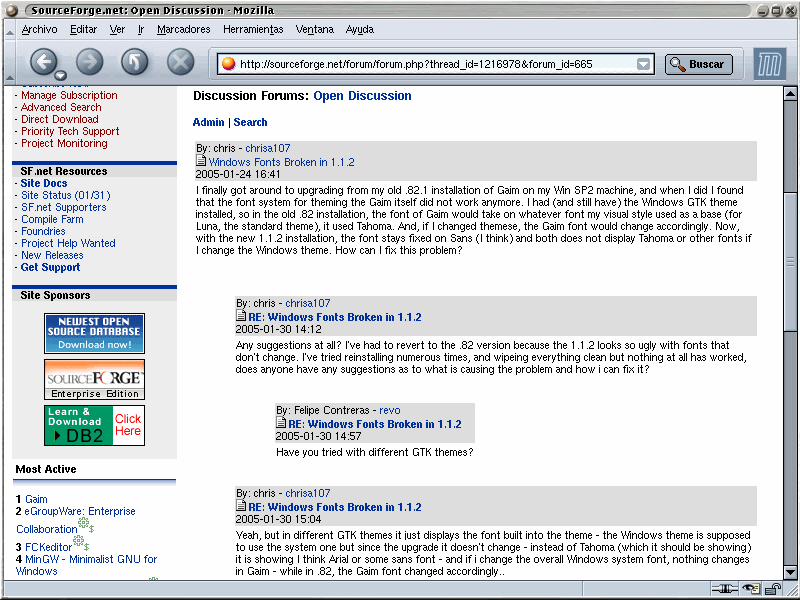
\includegraphics[bb=0 0 800 600, width=12cm, keepaspectratio]{img/foro2}
    \caption{Página con mensajes de un hilo}
    \label{figura:foro_msgs}
 \end{figure}


\subsection{Sistema de seguimiento de errores de Debian}
\label{intro_BTS}

El Proyecto Debian lo componen una agrupación de personas que comparten
la motivación de crear un sistema operativo libre basado en linux, haciendo
uso de herramientas creadas por el proyecto GNU. Debian hace gala de ser
distribución de linux de lo más completa ---con más de 8700 paquetes---,
dinámica ---con cientos de voluntarios que ayudan a hacerla evolucionar---,
y libre de ser usada y distribuida.

La distribución Debian posee un sistema de seguimiento de errores
(o \textit{Bug Tracking System} - BTS) que almacena informes detallados
de fallos comunicados por usuarios o desarrolladores.
En concreto, cada informe mantiene detalles
de un fallo, comprendiendo: título, estado del fallo (abierto-cerrado),
nivel de gravedad, etiquetas, dirección de quien abrió el informe y del
mantenedor\ldots Parte de estos parámetros son establecidos al avisar del
error, aunque modificables por un desarrollador escribiendo a
\texttt{control@bugs.debian.org}.
\\[0.5cm]
En cuanto a su funcionamiento básico, cuando un usuario descubre un fallo
en software procedente de paquetes mantenidos por Debian, procede a enviar
un informe sobre fallos en un mensaje
de correo a \texttt{submit@\-bugs.debian.org}. El sistema de seguimiento de fallos
considera abierto el informe y le asigna un número identificador,
que será comunicado al usuario y
el informe remitido tanto a la lista de correo \texttt{debian-bugs-dist} como
al mantenedor del paquete, siempre que sea conocido.

Si un desarrollador decide responder a un informe que le fue remitido, basta
con dirigir un correo a quien abrió el informe y a la dirección
\texttt{nºfallo@bugs.debian.org}. A continuación, el sistema de seguimiento
recibe dicho mensaje en \texttt{nºfallo@\-bugs.debian.org}, siendo archivado
junto al resto del informe y reenviado tanto al mantenedor del paquete como
a la lista de correo (\texttt{debian-bugs-dist}). Pero también existen
alternativas a este flujo de mensajes: un desarrollador puede comunicar
explícitamente con quien abrió el informe usando
\texttt{nºfallo-submitter@\-bugs.debian.org};
o bien, si la respuesta no es adecuada para la lista de correo, escribir a
\texttt{nºfallos\--quiet@\-bugs.debian.org} o
\texttt{nºfallos\--maintonly@\-bugs.debian.org}. Dirigiendo el mensaje a esta
última dirección, será archivado y enviado sólo al mantenedor del paquete;
en otro caso, únicamente será archivado.

Cuando el problema ha sido corregido, esto es, una vez almacenado en el archivo
de Debian un paquete incluyendo la corrección al error, el informe ha de
cerrarse. Por norma general, un informe sólo puede ser cerrado por quien lo
envió y por el mantenedor del paquete al que se hace referencia en el informe.
El método para cerrar los informes de fallo consiste en enviar un mensaje a
\texttt{nºfallo-done@\-bugs.debian.org}, donde el cuerpo del mensaje especifique
cómo fue resuelto el error. Este mensaje también será recibido por aquel quien
abrió el informe y la lista de correo \texttt{debian-bugs-closed}. Por último,
la persona que cierra el informe, la que lo abrió y la lista de correo reciben
sendas notificaciones indicando el cambio de estado del informe.


\subsection{Listas de correo en Mailman} \label{intro_listas}
Para empezar, introducimos unas notas acerca de las listas de correo así como
del software administrador de listas de correo Mailman.

Las listas de correo electrónico son listas formadas por direcciones de correo
de las personas que la integran. Su funcionamiento es simple: todo aquel
inscrito en una, recibe en su buzón de correo los mensajes que los participantes
de la lista remiten a ésta; de igual modo, toda persona suscrita puede dirigir
mensajes a la lista y éstos serán distribuidos entre los integrantes.
Son también conocidas como listas de discusión, ya que cualquier mensaje
enviado a una de éstas puede ser contestado por cualquier otro miembro
de la lista, con lo que se establece un intercambio de información.
De modo general, cada una de ellas está destinada a un tema bien definido,
permitiendo agrupar los contenidos relativos a un determinado contexto,
con lo que el usuario accede y aporta exactamente a donde pretende.

Por su parte, Mailman es un software ampliamente extendido para la administración
de listas de correo electrónico. Se trata de un software libre, escrito casi
en su totalidad en Python, y que destaca sobre otros programas con funciones
similares ---como Majordomo o SmartList--- por incorporar una interfaz web fácil
de usar para la administración de las listas. Su funcionalidad básica es la
de procesar los mensajes entrantes, y dependiendo de su contenido, actuar en
consecuencia sobre ellos y/o distribuirlos a los miembros de la lista determinada.
Además, incorpora características como filtros para evitar correo indeseado,
archivo de mensajes, restricciones de acceso a listas y archivos, etc.

Como se comentó en el apartado~\ref{SLE}, en el estudio cuantitativo de los
proyectos de software libre se ha de analizar, además del estado actual, la
evolución de los mismos en el pasado. Mailman facilita esta tarea al prestar
servicios de archivo de mensajes, en diferentes formatos y organizados según
ciertas prioridades. Así, para una lista de correo gobernada por Mailman,
se ofrecen archivos que compilan los mensajes enviados a la lista pertenecientes
a cada mes del año ordenados por: hilo (aparecen anidadas las respuestas a
cada mensaje), asunto (muestra de forma consecutiva enlaces a mensajes con
el mismo asunto), fecha (presenta enlaces a mensajes según el orden de llegada)
o autor. El principal inconveniente que plantea el formato en que se representan
estos archivos ---a la hora de analizar la lista--- es que fue pensado para
navegar a través de los diferentes mensajes: cada correo se encuentra en una
página web distinta, siendo posible acceder a mensajes anterior y siguiente
a través de sendos hiperenlaces. Afortunadamente para nuestros propósitos,
Mailman almacena la sucesión de correos mensuales en un único archivo de
texto plano, siguiendo el formato mbox. A grandes rasgos, en mbox
los mensajes de correo son representados según el estándar propuesto en la
RFC 2822, con la peculiaridad de estar delimitados por una línea inicial
'From ' y otra final en blanco (aunque existen variantes). En fin, más
adelante se profundizará en la estructura de estos archivos, elegidos para
extraer la información de interés en el estudio de listas de
correo asociadas a proyectos de software libre.

A modo de ejemplo, el siguiente texto muestra un fragmento de un archivo
con formato mbox:

{\footnotesize
\begin{verbatim}
    From gaurav at gold-solutions.co.uk  Fri Jan 14 14:51:11 2005
    From: gaurav at gold-solutions.co.uk (gaurav_gold)
    Date: Fri Jan 14 19:25:51 2005
    Subject: [Mailman-Users] mailman issues
    Message-ID: <003c01c4fa40$1d99b4c0$94592252@gaurav7klgnyif>

    Dear Sir/Madam,
    How can people reply to the mailing list?  How do i turn off
    this feature? How can i also enable a feature where if someone
    replies the newsletter the email gets deleted?
    Thanks

    From msapiro at value.net  Fri Jan 14 19:48:51 2005
    From: msapiro at value.net (Mark Sapiro)
    Date: Fri Jan 14 19:49:04 2005
    Subject: [Mailman-Users] mailman issues
    In-Reply-To: <003c01c4fa40$1d99b4c0$94592252@gaurav7klgnyif>
    Message-ID: <PC173020050114104851057801b04d55@msapiro>

    gaurav_gold wrote:
    >How can people reply to the mailing list?  How do i turn off
    this feature? How can i also enable a feature where if someone
    replies the newsletter the email gets deleted?

    See the FAQ
    >Mailman FAQ: http://www.python.org/cgi-bin/faqw-mm.py
    article 3.11
\end{verbatim}
}



\section{Python}
Python es un lenguaje de \textit{scripting} orientado a objetos. Proporciona
la simplicidad y facilidad de uso de un lenguaje interpretado, así como las
más avanzadas herramientas de programación propias de lenguajes destinados al
desarrollo de sistemas (como C o C++). Destaca por su facilidad de aprendizaje
y su portabilidad entre las distintas plataformas, tan sólo condicionada a
la presencia de un intérprete disponible.

Nombremos algunas de las propiedades que caracterizan a Python como lenguaje
de alto nivel:
\begin{itemize}
\item Tipado dinámico y fuertemente tipado. No requiere que nos tomemos la
molestia de declarar variables ya que reconoce su tipo desde que se asigna
un valor por primera vez. Eso sí, durante el tiempo de vida de una variable
ésta sólo puede pertenecer a un tipo. 
\item Proporciona estructuras de datos flexibles y sencillas de usar como
listas, diccionarios y strings, como parte intrínseca al lenguaje. Para
procesar cada uno de estos tipos de objeto, incorpora un conjunto de operaciones
que ahorrarán tiempo y esfuerzo al implementar tareas de uso habitual como
ordenaciones, búsquedas, etc.
\item Python posee una amplia colección de librerías dedicadas a tareas
específicas.
\item Administra automáticamente la gestión de memoria. Se encarga de
solicitar memoria en la creación de objetos y de liberarla cuando no van a
volver a ser utilizados.
\item Permite la construcción de sistemas de gran tamaño al incorporar
herramientas como clases, módulos, y excepciones.
\item A los programas escritos en Python pueden integrarse componentes
escritos en otros lenguajes. Por ejemplo, mediante el API de Python/C,
un código Python puede extender su funcionalidad incorporando componentes
escritos en C o C++, lo cual convierte a Python en un lenguaje de prototipado
rápido: las aplicaciones pueden ser implementadas en primera instancia con
Python para aumentar su velocidad de desarrollo y posteriormente ciertas
partes reescritas en C por motivos de eficiencia.
\end{itemize}

Con Python es perfectamente viable el desarrollo de proyectos software de gran
entidad, ejemplo de ello son el servidor de aplicaciones \textit{Zope} y el
sistema de intercambio de ficheros \textit{BitTorrent}, incluyendo al propio
\textit{Mailman}.

Otro aspecto que nos interesa particularmente es la incorporación, dentro de
la completa librería que ofrece, de módulos que manejan estándares comunes
en Internet (HTML, FTP, XML, HTTP, \ldots) y APIs para la comunicación con
bases de datos (para gestores como PostgreSQL, Oracle o MySQL).

A continuación hacemos mención a otro recurso que Python nos brinda y que
será de gran utilidad durante la implementación de este proyecto: las expresiones
regulares.


\subsection{Expresiones regulares} \label{regex}
Estrictamente aplicado a este campo, una expresión regular es un patrón
escrito en una sintaxis compacta y bastante críptica que se corresponde con
un conjunto de cadenas de caracteres (en adelante \textit{strings}).
Python proporciona un módulo especializado para procesarlas.

Las expresiones regulares se componen de caracteres especiales, que permiten
desde representar cualquier carácter salvo fin de línea ('.') o la repetición
en una
o más ocasiones de la expresión regular predecesora ('+'), hasta indicar
que existe
correspondencia sólo si una expresión regular va inmediatamente precedida de
otra en concreto. Así pues, mediante la combinación de metacaracteres se
puede simbolizar un número de conjuntos de strings prácticamente ilimitado.

Una vez definido un patrón pueden realizarse diferentes operaciones aplicadas
sobre un string. A través del módulo \textit{re} de Python se tiene acceso a
métodos que buscan posibles coincidencias del patrón en del string, permitiendo,
si la comparación tuvo éxito, obtener las posiciones de inicio y final del
substring coincidente. Existen otros métodos que segmentan el string en rodajas
delimitadas por el patrón o sustituyen las partes del string coincidentes
con el patrón.
El módulo aporta, además, facilidades para el manejo de grupos, que delimitan
zonas dentro del patrón que podrán ser recuperadas a posteriori. Esto será
de gran utilidad en caso de que sea necesario obtener un texto cuyo entorno
sea cambiante.

Como puede desprenderse de lo comentado, las expresiones regulares aportan
una gran potencia al manejo de strings dentro de un lenguaje de programación.
A pesar de ello, emplearlas para tareas en las que no son estrictamente
necesarias, aparte de ser un mal hábito, va en detrimento de la claridad del
código, complica sobremanera su depuración y repercute negativamente sobre su
eficiencia.




\newpage
\chapter{Objetivos}
\section{Descripción del problema}
Este proyecto puede considerarse ligado a uno más grande que pretende potenciar
una rama de la ingeniería del software: la ingeniería del software libre.
Ésta pretende aprovechar la existencia de una ingente cantidad de información
accesible derivada de las formas de desarrollo abiertas (código fuente,
comunicaciones entre desarrolladores, etc.) que llevan
a cabo los proyectos del software libre, de manera que puedan ser cuantificados,
medidos y estudiados. Los resultados y su consiguiente análisis ayudarán
enormemente en la comprensión de los fenómenos asociados a la
generación del software libre, al tiempo que facilitarán la toma de deciones
a partir de la experiencia adquirida.

Con el fin de crear unas herramientas esenciales que permitan disponer del
análisis de la mayor cantidad de proyectos posibles, el Grupo de Sistemas
y Comunicaciones de la universidad (GSyC) está desarrollando un macroproyecto
denominado Libre Software Engineering.

El presente proyecto se centra en la recopilación de datos relevantes producidos
durante el desarrollo de los proyectos de software libre, quedando al margen
el posterior examen de éstos. Como objetivo propone la elaboración de una
herramienta que sirva de base para la creación de utilidades de extracción
específicas a cada tipo de fuente de información. Se requiere, además, la
creación de tres de esas aplicaciones especializadas, con el fin de extraer
los parámetros de interés desde archivos de listas de correo (generados por
Mailman), el sistema de seguimiento de errores de Debian, y foros web de
proyectos alojados en SourceForge.

Estas utilidades han sido desarrolladas usando Python como lenguaje
de programación, basando la captación de la información de interés
en la comparación de patrones. Una información, que ha de ser agrupada y
empaquetada en un formato flexible y no adscrito a ninguna de las distintas
herramientas de extracción o de análisis.

\begin{figure}[H]
  \centering
  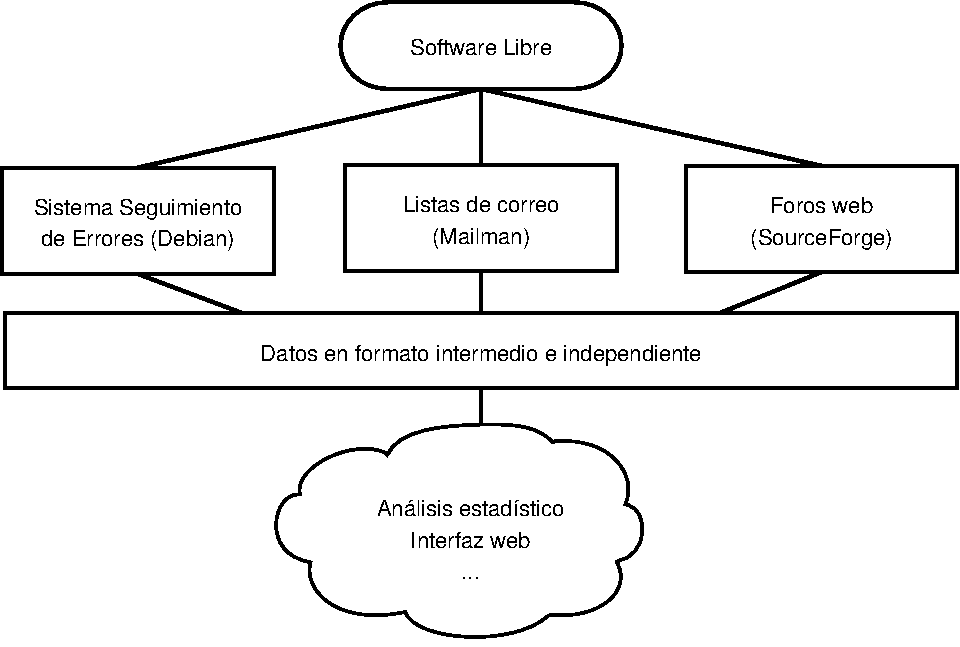
\includegraphics[width=14cm, keepaspectratio]{img/descrip}
  \label{figura:descript}
\end{figure}



\section{Requisitos}
El proyecto deberá cumplir ciertos requisitos básicos:
\begin{itemize}
\item Definir una interfaz unificado para herramientas futuras.
\item Almacenar resultados en formato intermedio para su posterior análisis:
  base de datos relacional y/o XML.
\item Proceso automatizado al máximo.
\item Fácil puesta en marcha y actualizaciones.
\item Tiempo de extracción de datos no será crítico.
\end{itemize}


\section{Modelo de desarrollo} \label{modelo}
Para el desarrollo de cualquier proyecto de software se realizan una serie de
tareas entre la idea inicial y el producto final. Ese desarrollo sigue una
determinada metodología o modelo de desarrollo, el cual
establece el orden en el que se llevan a cabo las tareas en el proyecto y
nos provee de requisitos de entrada y salida para cada una de las actividades.

El desarrollo de este proyecto se ha basado en un modelo de desarrollo
en espiral. Se optó por este modelo ya que fue diseñado para amoldarse a
productos que evolucionan con el tiempo, permitiendo definir etapas donde
nuevos objetivos y dificultades son añadidos de forma progresiva. Además,
resulta un modelo muy flexible a requisitos cambiantes, ya que en posteriores
iteraciones el producto puede ir adaptándose a las nuevas necesidades.

El modelo en espiral ofrece también la posibilidad de ir construyendo
prototipos que surgen como producto final de cada ciclo de la espiral,
y tienen como finalidad la de evaluar el cumplimiento de los requisitos
definidos durante la correspondiente iteración. La creación de prototipos
se ajusta perfectamente a las características de este proyecto, pues
podremos tantear ante situaciones reales su correcto funcionamiento.
Estos prototipos fueron desarrollados, pues, de forma incremental basándonos
en el anterior (siempre que éste superase las pruebas), incorporando nuevas
funcionalidades. Esto garantiza que las funciones básicas resulten extensamente
probadas.

El conjunto de actividades en que se divide el modelo de desarrollo escogido
hubo de ser adaptado a la dimensión del proyecto, dando lugar a las siguientes
fases:
\begin{itemize}
\item \textbf{Comunicación con el cliente}. El cliente especifica los objetivos
del ciclo de la espiral. Se corresponde con una reunión donde el tutor del
proyecto pone en conocimiento del autor del mismo los requisitos de cada ciclo.
Unos requisitos funcionales y estructurales que, aunque generales, siempre
precisos, dado que no tratamos con un cliente convencional.
\item \textbf{Planificación}. Se definen recursos, tiempo y otros parámetros
relacionados con la presente iteración. De nuevo proporcionadas por el tutor
a tenor del resultado de evaluar el prototipo correspondiente a la iteración
previa.
\item \textbf{Construcción y adaptación}. El sistema es desarrollado.
Engloba tareas como el diseño y la implementación, ampliamente comentadas en
el próximo capítulo.
\item \textbf{Pruebas}. Se confirma que los requisitos se cumplen satisfactoriamente.
Se remitió al tutor tanto el prototipo como los resultados de las pruebas
aplicadas sobre éste.
\end{itemize}

Cabe destacar que aunque los distintos analizadores de fuentes de información
se presenten como desarrollados en paralelo, este hecho no se corresponde
estrictamente con la realidad. Sin embargo, al haber evolucionado de modo
similar, se prefiere no complicar innecesariamente la exposición.

La fase de pruebas no se incluirá en la documentación por falta de espacio
para desarrollar casos suficientemente representativos.




\newpage
\chapter{Diseño e implementación}

\section{Arquitectura general} 
\label{arquitectura}

El primer objetivo que planteamos satisfacer es la creación de un \textit{parser}
básico cuya función sea extraer los parámetros a estudiar a partir de un documento.
Esta utilidad analizadora recibe por parte del usuario argumentos necesarios
para su funcionamiento. El principal es la URL que direcciona el documento a
examinar, junto con diversos parámetros que configuran aspectos relacionados
con la base de datos donde depositar los resultados.

El funcionamiento de la unidad Parser consiste en recoger la petición compuesta
por los parámetros citados, solicitar la información correspondiente a la URL,
analizarla para obtener los datos cuantificables de interés, y agruparlos con la
finalidad de que permanezcan alojados en una base de datos.
Su composición interna puede dividirse, por tanto, en las tres subunidades
dedicadas que se muestran en la figura~\ref{figura:arquitectura}.

\begin{figure}[H]
  \centering
  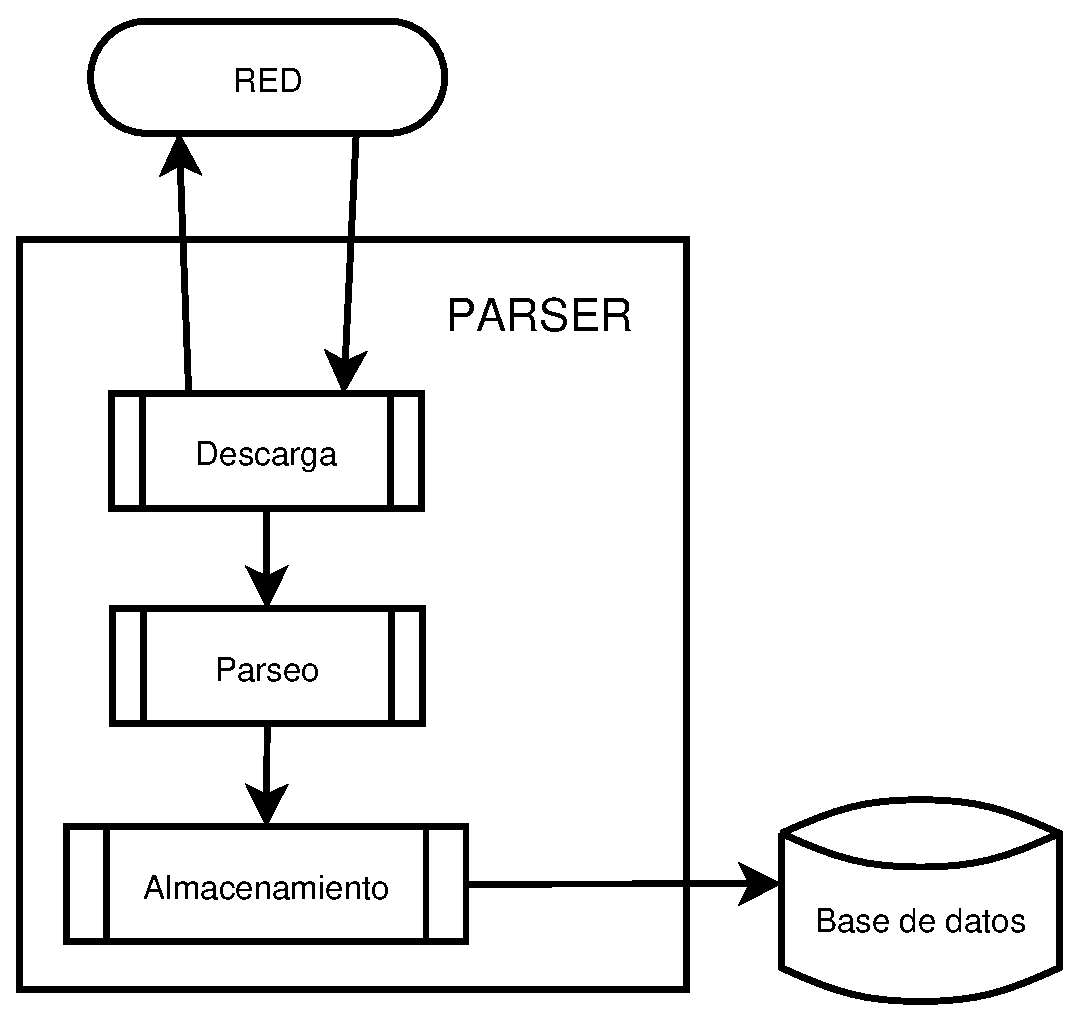
\includegraphics[width=9cm, keepaspectratio]{img/arquitectura}
  \caption{Estructura del parser básico}
  \label{figura:arquitectura}
\end{figure}

Con el \textit{parser} genérico ---que hará las veces de interfaz---
ya definido, se procederá a desarrollar analizadores derivados del anterior
y especializados en la extracción de datos desde fuentes de información
sobre la evolución de proyectos de software libre. Los \textit{parsers}
obtenidos serán independientes entre sí y dedicados en exclusiva a un tipo
de fuente. Aún más, se diseñarán para \textit{parsear} un único modo de
representación de entre los que pone a nuestra disposición un tipo de fuente
concreto.

Así, se desarrollará un \textit{parser} que trate los foros web de SouceForge
partiendo de la página inicial del foro de un proyecto cualquiera, siempre
que los enlaces a los distintos hilos se ordenen del modo adecuado (\textit{Ultimate}).
Otra extensión del \textit{parser} básico se encargará de los archivos de
listas de correo confeccionados por Mailman, enlazados desde una única página
donde se encuentran ordenados por fecha.
Para finalizar, los informes de fallos procedentes del sistema de gestión de
errores de Debian serán tratados por un tercer analizador, capturando desde
la secuencia de mensajes en bruto que llegan a dicho sistema.

\begin{figure}[H]
  \centering
  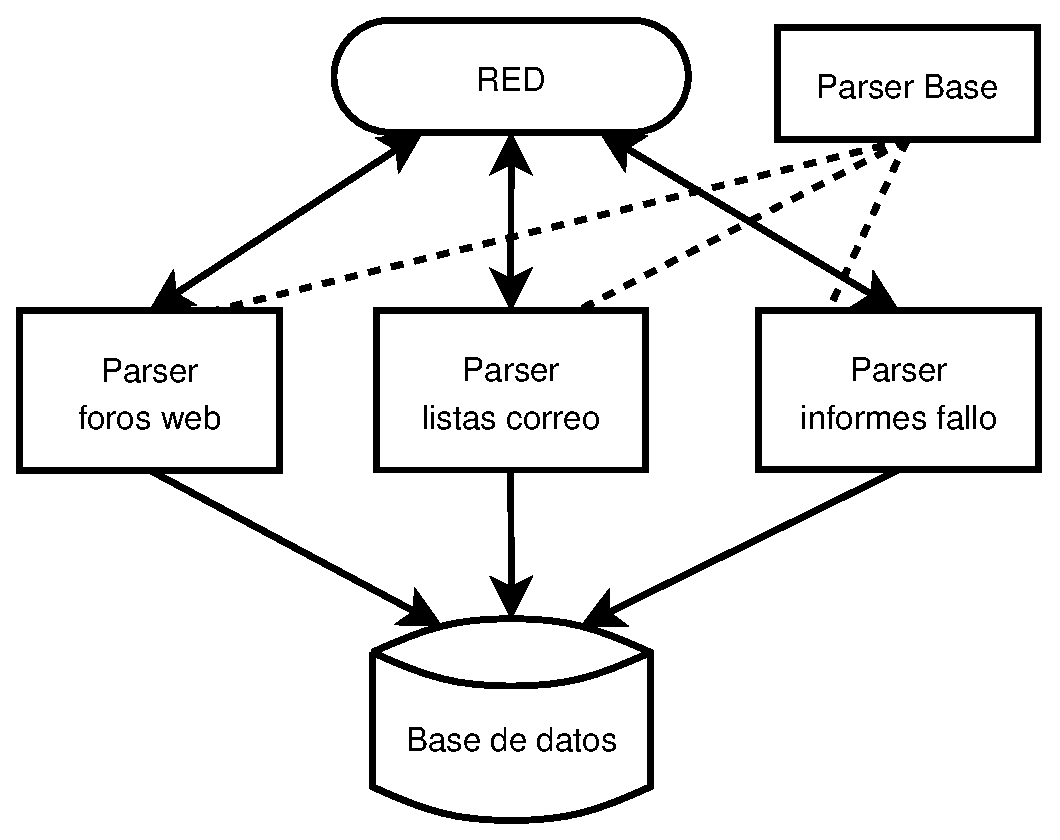
\includegraphics[width=9cm, keepaspectratio]{img/arquitectura2}
  \caption{Esquema del proyecto en su conjunto}
  \label{figura:arquitectura2}
\end{figure}

El desarrollo de los componentes mencionados, como es deducible de lo
expuesto en el apartado~\ref{modelo}, se hará de manera incremental,
dividiéndolo en distintas iteraciones en cada una de las cuales se dará lugar
a un prototipo basado en el resultante de la iteración previa. Así resultará:
\begin{itemize}
\item \textbf{Iteración 0}. Una fase previa que se limitará al estudio de la
estructura de los diferentes documentos a \textit{parsear}. En realidad se
trata de un paso anterior al desarrollo y, por tanto, no implica un avance en
la espiral ni desemboca en un prototipo, pero la vital importancia de esta labor
nos obliga a dedicarle un lugar destacado en la evolución del proyecto.
\item \textbf{Iteración 1}. Una primera fase cuyo objetivo es la creación del
\textit{parser} básico que establecerá una interfaz común para el resto de
sus homónimos derivados de éste.
\item \textbf{Iteración 2}. Una segunda fase que pretende extender la funcionalidad
del \textit{parser} generado en la fase anterior y crear especializaciones
adaptadas a las tres fuentes de información mencionadas de forma recurrente
a lo largo del presente documento.
\item \textbf{Iteración 3}. Una última fase donde se añadirá la capacidad de
realizar actualizaciones incrementales a los \textit{parsers} resultantes de
la iteración anterior.
\end{itemize}



\section{Iteración 0. Estudio previo}
Dedicaremos ahora unas palabras a la descripción exhaustiva de los formatos
en que vienen representados los documentos a analizar (en adelante \textit{parsear},
para evitar confunsiones con el propio análisis y procesado del conjunto de
parámetros ya almacenados).


\subsection{Foro web}
Como se anticipó en el apartado~\ref{intro_foros}, los foros de SourceForge
únicamente son ofrecidos en HTML para disfrute de todo aquel que se valga de un
navegador web para visitarlos. Si además unimos a esto que no siguen un esquema
estándar, el cual puede variar en cualquier momento sin que se detalle qué fue
modificado (gracias a que son generados por herramientas no libres; por cierto,
llegó a suceder durante el desarrollo del proyecto), nos vemos obligados a
estudiar su estructura mediante la observación del propio código HTML.

Como también se comentó anteriormente, el proceso de \textit{parseo} de un foro
completo se iniciará desde la página de inicio de éste en modo \textit{Ultimate}.
Esa página inicial se compone de una sucesión de títulos de hilos (con su
correspondiente hiperenlace a la página que muestra el hilo), junto con el autor
del mensaje inicial, número de respuestas y la fecha del último mensaje enviado
(la cual se emplea para ordenar de forma descendente los hilos). Hacia el final
de la página se encuentra un hiperenlace a otra página de similares
características donde aparecen los siguientes hilos.
La estructura de este tipo de páginas (valga como ejemplo la de la figura
\ref{figura:foro_hilos}) se muestra a continuación.

{\scriptsize
  \begin{verbatim}
 <! -- Código de publicidad -->
 <! -- Código de barras de navegación -->
 <! -- Código de columna izquierda -->
 <! -- Inicio código de columna derecha -->
 [...]
 <TABLE WIDTH="100%" BORDER="0" CELLSPACING="1" CELLPADDING="2">
   <TR BGCOLOR="">
     <TD ALIGN="MIDDLE"><FONT COLOR=""><B>Topic</B></FONT></TD>
     <TD ALIGN="MIDDLE"><FONT COLOR=""><B>Topic Starter</B></FONT></TD>
     <TD ALIGN="MIDDLE"><FONT COLOR=""><B>Replies</B></FONT></TD>
     <TD ALIGN="MIDDLE"><FONT COLOR=""><B>Last Post</B></FONT></TD></TR>
       <!-- Inicio de item -->
       <TR BGCOLOR="#FFFFFF"><TD><A HREF="DIRECCION_DEL_HILO>                     ->
         <IMG src="RUTA_IMAGEN" border="0" alt="" width="15" height="13">  &nbsp; ->
         <B>TITULO DEL HILO</A></TD><TD><a href="DIR_CUENTA_USUARIO">USUARIO</a>  ->
         </TD><TD>NUM_RESPUESTAS                                                  ->
         </TD><TD>FECHA DE ENVIO DEL ULTIMO MENSAJE (YYYY-MM-DD HH:MM)</TD></TR>
       <!-- Fin de item -->
       [...]
       <!-- Inicio de item -->
       <TR BGCOLOR="#FFFFFF"><TD><A HREF="DIRECCION_DEL_HILO>                     ->
         <IMG src="RUTA_IMAGEN" border="0" alt="" width="15" height="13">  &nbsp; ->
         <B>TITULO DEL HILO</A></TD><TD><a href="DIR_CUENTA_USUARIO">USUARIO</a>  ->
         </TD><TD>NUM_RESPUESTAS                                                  ->
         </TD><TD>FECHA DE ENVIO DEL ULTIMO MENSAJE (YYYY-MM-DD HH:MM)</TD></TR>  ->
       <!-- Fin de item -->
         </TABLE><TABLE WIDTH="100%" BORDER="0">
   <TR BGCOLOR="#EEEEEE"><TD WIDTH="50%">&nbsp;</TD><TD>&nbsp; ->
     </TD><TD ALIGN="RIGHT" WIDTH="50%">                       ->
     <FONT face="Arial, Helvetica" SIZE=3 STYLE="text-decoration: none"><B>
   <A HREF="DIRECCION_DE_PROXIMA_PAGINA">
   <B>Next Messages [...]</A></TABLE>[...]
 [...]
 <!-- Fin de columna derecha -->
 <!-- Fin de documento -->
\end{verbatim}
}

Si se siguen los enlaces se alcanzan las páginas que
contienen los mensajes de cada hilo. Este tipo de página muestra una sucesión
de mensajes, compuestos por una \textit{cabecera} que registra el nombre del
usuario que lo envió, su alias, asunto del mensaje y fecha de recepción; y por
un cuerpo que alberga el contenido del propio mensaje. Como puede observarse
en la figura~\ref{figura:foro_msgs}, los mensajes aparecen alineados a distinta
profundidad conforme sean respuesta o no a comentarios previos.
Las páginas con los mensajes de todo un hilo siguen estructura genérica:

{\scriptsize
\begin{verbatim}
 <! -- Código de publicidad -->
 <! -- Código de barras de navegación -->
 <! -- Código de columna izquierda -->
 <! -- Inicio código de columna derecha -->
 [...]
   <!-- Inicio de mensaje -->
   <TABLE BORDER="0"><TR><TD BGCOLOR="#DDDDDD" NOWRAP>By: NOMBRE_USUARIO - <    ->
      a href="CUENTA_USUARIO">NICK_USUARIO</a><BR>
      <A HREF="/forum/message.php?msg_id=ID_MENSAJE"><IMG src="RUTA_IMAGEN"     ->
         border="0" alt="" width="10" height="12"> ASUNTO DE MENSAJE</A> &nbsp; ->
         <BR>FECHA DE RECEPCION DEL MENSAJE (YYYY-MM-DD HH:MM)
      </TD>
      </TR><TR><TD>CUERPO DEL MENSAJE<br /><br /></TD></TR></TABLE><P>
   <!-- Fin de mensaje -->
   [...]
   <!-- Inicio de mensaje -->
   <TABLE BORDER="0"><TR><TD BGCOLOR="#DDDDDD" NOWRAP>By: NOMBRE_USUARIO - <    ->
      a href="CUENTA_USUARIO">NICK_USUARIO</a><BR>
      <A HREF="/forum/message.php?msg_id=ID_MENSAJE"><IMG src="RUTA_IMAGEN"     ->
         border="0" alt="" width="10" height="12"> ASUNTO DE MENSAJE</A> &nbsp; ->
         <BR>FECHA DE RECEPCION DEL MENSAJE (YYYY-MM-DD HH:MM)
      </TD>
      </TR><TR><TD>CUERPO DEL MENSAJE<br /><br /></TD></TR></TABLE><P>
   <!-- Fin de mensaje -->
   <TABLE WIDTH="100%" BORDER="0">
   <TR BGCOLOR="#EEEEEE"><TD WIDTH="50%">&nbsp;</TD><TD>&nbsp;</TD>             ->
      <TD ALIGN="RIGHT" WIDTH="50%">&nbsp;</TABLE>[...]
 [...]
 <!-- Fin de columna derecha -->
 <!-- Fin de documento -->
\end{verbatim}
}

Hay que matizar que en el esquema no se han incluido las etiquetas destinadas
a generar los niveles de profundidad de los mensajes, aunque habrán de
considerarse en un futuro. Para ser precisos, es por medio de listas de elementos
no ordenadas y anidadas como se consigue este efecto, esto es, se sitúan entre
los mensajes las etiquetas de apertura y cierre \texttt{UL} necesarias.

En ciertas ocasiones el modelo descrito no se respeta por completo,
apareciendo, por ejemplo, las líneas de asunto en negrita.


\subsection{Archivo de lista de correo}
Los archivos de listas de correo creados por Mailman siguen el formato mbox,
como se mencionó en el apartado~\ref{intro_listas}. En mbox
los mensajes de correo siguen el estándar propuesto en la
RFC 2822, aunque aparecen delimitados por una línea inicial
'From ' y otra final en blanco (aunque existen variantes).

Antes de proceder a la recogida de datos de este tipo de documento,
resultará interesante conocer las cabeceras que componen los
mensajes adaptados a la RFC 2822, pues de ellas se extraerá valiosa
información sobre el mensaje.

He aquí las cabeceras más comunes:
\begin{itemize}
\item
From: especifica la dirección de correo(mailbox) de el/los responsable(s)
de escribir el mensaje.
\item
Sender: especifica la dirección del responsable de la última transmisión
del mensaje. Si coincide con la aparecida en campo 'From', debe omitirse.
\item
Reply-To: si está presente, indica la(s) dirección(es) donde el autor del
mensaje sugiere que se le envíen las respuestas.
\item
To: contiene la(s) dirección(es) de los destinatarios principales.
\item
Cc: contiene las direcciones de otros destinatarios que recibirán el mensaje
aunque el contenido de éste no vaya dirigido a ellos.
\item
Bcc: contiene las direcciones de destinatarios del mensaje cuyas direcciónes
no deben ser reveladas al resto de destinatarios.
\item
Subject: contiene una descripción del tema que trata el mensaje.
\item
Received: alberga dirección de máquina intermedia a través de la que se
transmitió el mensaje, acompañado de la fecha de retransmisión.
\item
Message-ID: identificador único de una versión concreta de cada mensaje.
Unicidad garantizada por el host emisor.
Fácilmente interpretable para las máquinas aunque no para las personas.
\item
msg-id: identificador único (global) del mensaje.
\item
In-reply-to: almacena el identificador del mensaje al que el actual responde
\item
References: almacena identificadores (Message-ID) del resto de mensajes que
constituyen el hilo de conversación.
\end{itemize}

A continuación se muestran las cabeceras que encontraremos en las listas de
correo de este estilo, junto con su estructura típica:

{\scriptsize
\begin{verbatim}
From USUARIO en/at DOMINIO  DIA(Mon,Tue,Wed,...) MES(Jan,Feb,Mar,...)  D HH:MM:SS YYYY
From: USUARIO en/at DOMINIO (AUTOR)
Date: DIA(Mon,Tue,Wed,...) MES(Jan,Feb,Mar,...)  D HH:MM:SS YYYY
Subject: [NOMBRE_LISTA] ASUNTO
In-Reply-To: <ID_MENSAJE_2>
References: <ID_MENSAJE_2> <ID_MENSAJE_3>
Message-ID: <ID_MENSAJE>

\end{verbatim}
}

Si además de lo anteriormente comentado, conocemos que ciertas cabeceras pueden
ocupar varias líneas y que los nombres de campos pueden presentarse tanto en
mayúsculas como en minúsculas indistintamente, estaremos en disposición de iniciar
la creación del \textit{parser} para los archivos de listas de correo.


\subsection{Informe de error}
Toda vez explicado el flujo de mensajes (revisar el apartado~\ref{intro_BTS})
producido desde el momento de apertura al de cierre de un informe de fallo en el
sistema de seguimiento de errores de Debian, nos es imprescindible documentar
los diversos modos de acceso a los registros que detallan la evolución de los
errores.

Están disponibles métodos que permiten el acceso a los registros a
través de la web o mediante correo electrónico. A pesar de que este último
procedimiento es tan sencillo de realizar como enviar un mensaje de correo
electrónico a \texttt{request@bugs.debian.org} cuyo contenido se valga de un
conjunto de órdenes que den forma a la petición, no es el método más
conveniente para nuestros fines.

Para ser exactos, queda otra alternativa que se ofrece es la de crear un
espejo local de todos los informes existentes. Quizá sea una opción a tener
en cuenta en el futuro.

En cuanto al acceso por web, se posibilita mediante la cumplimentación de un
formulario ---que descartaremos por no resultar cómodo--- o directamente
visitando URL que direcciona bien el informe de error
(\url{http://bugs.debian.org/id_informe}; formato HTML o mbox),
la página con enlaces a informes de error correspondiente a un determinado
paquete (\url{http://bugs.debian.org/paquete}),
la página con enlaces a informes de error de cierta gravedad
(\url{http://bugs.debian.org/tag:etiqueta}), etc.
Como pretendemos extraer la información de cada error sin complicaciones
innecesarias, desde un primer momento se eligió \textit{parsear} los informes
en formato mbox (direccionados como \url{http://bugs.debian.org/mbox:id_informe}).

Cada mensaje del archivo mbox presenta una serie de cabeceras, de entre las
que destacan las siguientes por facilitarnos los datos que buscamos:

{\scriptsize
\begin{verbatim}
From DIRECCION_REMITENTE DIA(Mon,Tue,Wed,...) MES(Jan,Feb,Mar,...) DD HH:MM:SS YYYY
Received: (at DESTINO) by bugs.debian.org; D MES(Jan,Feb,Mar,...) YYYY HH:MM:SS +0000
From: <DIRECCION_REMITENTE>
Subject: TITULO DE INFORME
To: DESTINO@bugs.debian.org
Message-Id: <ID_MENSAJE>
Date: DIA(Mon,Tue,Wed,...), DD MES(Jan,Feb,Mar,...) YYYY HH:MM:SS +XY00
...
\end{verbatim}
}

Procedemos ahora a describir ciertos tipos de mensaje de cuyo cuerpo podremos
rescatar información de interés.

Todo mensaje que abre un informe es enviado a la dirección
\texttt{submit@\-bugs.\-debian\-.org}. El cuerpo de este mensaje se inicia con una
secuencia de pseudocabeceras, de las cuales \textit{package} y \textit{version}
son obligatorias (en teoría, porque el sistema de seguimiento de errores
aceptará mensajes sin ellas). Presentan este aspecto:

{\footnotesize
\begin{verbatim}
Package: PAQUETE CON FALLO
Version: VERSION DEL PAQUETE
Severity: GRAVEDAD
\end{verbatim}
}

Una línea en blanco tras ellas se describirá el problema que observó el usuario y
como fin de mensaje la mayor cantidad de detalles posibles para que mantenedor
del paquete consiga reproducir el error e intentar solucionarlo: texto completo
del mensaje de error, proceso seguido para mostrar el problema, detalles de la
configuración del programa que falla, versiones del paquete, kernel, etc.

Cada mensaje enviado a \texttt{control@\-bugs.\-debian.org} pretenderá modificar
el estado de un informe.
Su cuerpo contendrá una secuencia de órdenes y etiquetas finalizada por la orden
\textit{thank}, \textit{quit} o \textit{stop}.
Seguidamente puede añadirse cualquier comentario, que será ignorado por el sistema
de gestión de errores al procesarlo.
Estas órdenes realizan funciones como reabrir un informe de fallos en caso
de haber sido cerrado (\textit{reopen}), cambiar el título a un informe de
fallos (\textit{retitle}),
cambiar el paquete al que está asignado el error (\textit{reassign}),...;
siendo su sintaxis general (existen variantes a tratar):

{\footnotesize \begin{verbatim}<ORDEN ID_INFORME NUEVO_VALOR>\end{verbatim}}

a excepción de \textit{clone} y \textit{merge},
que respectivamente duplica un informe de error y fusiona dos o más informes
en uno, y siguen la forma:

{\footnotesize \begin{verbatim}<orden ID_INFORME ID_OTRO_INFORME>\end{verbatim}}

Por su parte, las etiquetas son atributos que referencian la situación del
error en la actualidad. Hay numerosas etiquetas: unas indican que el error
no ha podido ser reproducido por el mantenedor del paquete
(\textit{unreproducible}), otras avisan de que el error fue subsanado
(\textit{fixed}), otras advierten de que se ha encontrado la solución al fallo
y pronto será enviada (\textit{pending}), etc. Su estructura característica
es:

{\footnotesize \begin{verbatim}tag(s) ID_INFORME X TAG1 TAG2 TAGn\end{verbatim}}

donde X varía entre '+', '-', o '=' según se pretenda añadir, quitar o establecer
la serie de etiquetas.

El formato del archivo a \textit{parsear} posee multitud de peculiaridades que
deberemos tener en cuenta en el momento de crear el analizador, por lo que
conviene recurrir al código del \textit{parser}
donde todas aparecen comentadas junto al código que las trata.
La más visible de ellas es que los mensajes enviados a
\texttt{control@\-bugs.\-debian.org} aparecen repetidos tantas veces como líneas
de órdenes o etiquetas sean analizadas por el sistema de gestión de errores.



\section{Iteración 1. Creación de un \textit{parser} genérico}


\subsection{Diseño}
En esta primera fase o iteración se procederá a construir un \textit{parser}
básico. Hablamos de un \textit{parser} genérico capaz de analizar potencialmente
cualquier tipo de documento, aunque a efectos prácticos no reconoce ninguno
en particular, limitándose a proporcionar un interfaz para crear a posteriori
analizadores especializados en distintas clases de documentos.
En el apartado~\ref{arquitectura} ya se anticipó que la estructura de este
analizador básico se divide en tres subunidades, que denominamos \textit{Descarga},
\textit{Parseo} y \textit{Almacenamiento}.

La primera de ellas (\textit{Descarga}), tendrá por cometido establecer
conexión con la URL especificada y descargar su contenido. En un principio
podría suponerse que las fuentes de información a manejar se alojan en un
servidor remoto accesible a través de la red ---ciertamente es lo más probable---,
aunque podría darse el caso de disponer en una unidad de almacenamiento local
de una copia del archivo y pretender acceder a ella, de modo que se considerarán
ambas posibilidades. En cuanto a qué hacer con el documento una vez descargado,
podríamos optar por almacenarlo en disco a la espera de que otra subunidad lo
requiera; pero previendo que nuestro \textit{parser} no comenzará a tratar un
documento a menos que haya concluido su labor con el anterior, se prefiere
mantenerlo en memoria ya que su uso por parte de la subunidad \textit{Parseo}
será inmediato.

Respecto a la subunidad \textit{Parseo}, será la encargada de realizar la tarea
de extracción de la información requerida desde el documento obtenido por la
subunidad \textit{Descarga}. El proceso de \textit{parseo} que se llevará
a cabo plantea una división del documento en fragmentos que bien podrían ser
los mensajes a analizar, y un posterior análisis aplicado a cada uno de ellos
en busca de determinados parámetros, produciendo una ristra de estos parámetros
agrupados por fragmento. Esta forma de proceder viene determinada por la
naturaleza de las fuentes a analizar, y es que todas ellas suponen
una interaccion entre desarrolladores/usuarios por medio de mensajes.

El resultado de la subunidad \textit{Parseo} será tomado por \textit{Almacenamiento},
la cual insertará los datos recibidos en la(s) tabla(s) de la base de datos
indicada(s). Hay que tener en cuenta que los datos a recuperar variarán según
de qué fuente de información se pretendan extraer, con lo que no es viable
responsabilizar al usuario de la herramienta de la creación de la(s) tabla(s).
Es por ello que esta subunidad se encargará, además, tanto de la creación de
la base de datos como de la(s) tabla(s) a utilizar.


\subsection{Implementación}
El \textit{parser} genérico será implementado en Python como una clase,
denominada \texttt{Parser\-Class} y contenida en el módulo \texttt{parser.py}.
Que esté constituido como una clase aportará todas las propiedades que éstas
incorporan, permitiendo definir subclases que heredarán su interfaz y podrán
redefinir sus métodos y atributos. Esto habilitará la adaptación del \textit{parser}
al análisis de distintos tipos de documentos (hecho que ocurrirá en
próximas iteraciones), afectando principalmente a las operaciones que engloba
la subunidad \textit{Parseo}.

Dado que intensivo uso que se hará de la clase que implementa el \textit{parser}
genérico, hemos estimado oportuno la inclusión de piezas de código representativas,
aprovechando además los comentarios autoexplicativos que incorporan.

La funcionalidad de la subunidad \textit{Descarga} recaerá sobre el método
\texttt{download\_url}. Hace uso del módulo \texttt{urllib}, que nos proporciona
una capa de abstracción sobre varios protocolos utilizables para la obtención
de un archivo desde la red o un disco local (véase apartado~\ref{urllib}).

{\footnotesize
\begin{verbatim}
 def download_url (self, url):
     ' Descarga la web especificada '
     # 'url' : String identificador de la web
     #         o ruta de disco donde está almacenada.
     # Salida : Se devuelve su contenido a modo de string.
     
     import urllib
     url_dscrp = urllib.urlopen(url)
     print '\nDownloading... %s' % url
     self.code = url_dscrp.read()
     url_dscrp.close()
\end{verbatim}
}

En cuanto a la subunidad \textit{Parseo}, el paso del diseño a la implementación
será directo: la función de fragmentar el documento en mensajes delegará en el método
\texttt{split}; la función de búsqueda de los parámetros de interés, en el método
\texttt{analize}; y la aplicación del análisis sobre cada fragmento, en
\texttt{parse}. Debe destacarse, por otra parte, que estos métodos operarán
con expresiones regulares debido a la flexibilidad que éstas aportan,
colaborando así a cumplir con el requisito de generalidad del \textit{parser}.
Dicha generalidad se extiende a las funcionalidades de estos métodos,
pretendiendo que sea necesario sobreescribirlos en el menor número de ocasiones
posible (queda patente en los comentarios).

{\scriptsize
\begin{verbatim}
 def split (self, code, regex_begin, regex_end, include_begin=1, include_end=1):
     ' Divide texto en subpartes delimitadas por patrones de inicio y fin '
     # 'code' : String que contiene el código_html/texto_plano a dividir.
     # 'regex_begin' : Expresión regular coincidente con inicio de mensaje.
     # 'regex_end'   : Expresión regular coincidente con fin de mensaje.
     # Devuelve lista con mensajes seleccionados.

     ## Por defecto, línea de inicio y fin están incluidas ambas en el mensaje
     ## Línea inicial de un mensaje puede coincidir con línea final del próximo

     list_of_msgs, msg_data = [], 0
     for line in code.split('\n'):
         if not msg_data:
             if regex_begin.search(line):
                 # Línea de comienzo del mensaje
                 msg_data = 1
                 temp_msg = ''
                 if include_begin:
                     temp_msg = line + '\n'
         else:
             if regex_end.search(line):
                 # Línea de fin del mensaje
                 if include_end:
                     temp_msg += line
                 list_of_msgs.append(temp_msg)
                 msg_data = 0
                 if regex_begin.search(line):
                     msg_data = 1
                     temp_msg = ''
                     if include_begin:
                         temp_msg = line + '\n'
             else:
                 temp_msg += line + '\n'
     # Fin de texto sin encontrar fin de mensaje
     if msg_data:
         list_of_msgs.append(temp_msg)
     return list_of_msgs


 def analize (self, message, regexes, content_re = ''):
     ' A partir de un texto se obtienen elementos de interés '
     # 'message' : String que almacena mensaje a analizar.
     # 'regexes' : Tupla formada por pares (elemento buscado, expresión regular
     #             coincidente con entorno del elemento).
     # Devuelve diccionario: {key=elemento_buscado: value=valor_elemento_encontrado}

     ## Pueden encontrarse varios elementos por línea

     dict = {}
     ## Obteniendo contenido ##
     if content_re:
         s = content_re[1].search(message)
         index = s.start()
         dict[content_re[0]] = message[index:]
         message = message[:s.end()]
     res = list(regexes)
     for line in message.split('\n'):
         found = []
         for regex in res:
             match = regex[1].search(line)
             if match:
                 dict[regex[0]] = match.groups()[0]
                 found.append(regex)
         for regex in found:
             res.remove(regex)
     return dict


 def parse (self, code, regex_begin, regex_end, regexes, content_re='',
            incl_begin=1, incl_end=1):
     # 'code' : String que contiene el código_html/texto_plano a analizar.
     # 'regexes' : Tupla formada por pares (elemento buscado, expresión regular
     #             coincidente con entorno del elemento).
     # Retorna secuencia de diccionarios:
     #    {key=elemento_buscado: value=valor_elemento_encontrado}.
     self.data = []
     msgs = self.split (code, regex_begin, regex_end, incl_begin, incl_end)
     for msg in msgs:
         self.data.append( self.analize(msg, regexes, content_re) )
\end{verbatim}
}

Por último, las operaciones relacionadas con el manejo de la base de datos
quedarán englobadas dentro de la subunidad \textit{Almacenamiento}.
Se harán imprescindibles métodos que creen una base de datos e inserten
información en ella. \texttt{create\_database} será capaz de crear una base
de datos (en caso de que no exista previamente) y tantas tablas como se desee,
siempre que se le proporcione nombre y descripción de cada una.
Por su parte, a \texttt{feed\_database} le bastará con el nombre de la tabla
y una secuencia de filas (acepta una sola, pero está optimizado para inserción
múltiple) para insertarlas en la base de datos.

En cualquier operación de este tipo se empleará el módulo MySQLdb
(ver apartado~\ref{mysqldb}) para comunicar las peticiones realizadas al sistema
gestor MySQL. No se necesitará un gestor más completo o potente para el uso
que hará de la base de datos nuestra herramienta.

{\scriptsize
\begin{verbatim}
 def create_database (self, table_data):
     ' Crea base de datos y tabla(s) donde albergar resultados '
     # 'table_data' : tupla compuesta por parejas
     #                (nombre de tabla, estructura de tabla)
     
     db = MySQLdb.connect(host=self.host, user=self.user, passwd=self.password)
     c  = db.cursor()
     try:
         c.execute('CREATE DATABASE %s' % self.db)
     except _mysql_exceptions.ProgrammingError, e:
         print e
     c.close()
     db.close()
     # Reconexión
     db = MySQLdb.connect(host=self.host, user=self.user,
                          db=self.db, passwd=self.password)
     c  = db.cursor()
     try:
         for elem in table_data:
             c.execute ('CREATE TABLE %s (%s)' % (elem[0],elem[1]))
     except _mysql_exceptions.OperationalError, e:
         print e
     c.close()
     db.close()
     
     
 def feed_database (self, table_name, data):
     ' Introduce en una base de datos información seleccionada previamente '
     # 'table_name' : String que especifica el nombre de la tabla donde
     #                se recogerá la información.
     # 'data' : Datos a insertar en la tabla.
     #          Tupla compuesta por diccionarios: cada uno contiene info
     #          correspondiente a una fila de la tabla
     #          {key=columna : value=valor_columna}
     
     # Comprobando si lista con datos está vacía
     if not len(data):
         print 'Sin datos a introducir'
         return
     # Apertura de base de datos _ya existente_
     db = MySQLdb.connect(host=self.host, user=self.user,
                          db=self.db, passwd=self.password)
     c  = db.cursor()
     # -- Inserción de datos en tabla --
     # columns = lista de la forma [key1,key2,...,keyN]
     # values  = lista de la forma [%(key1)s,%(key2)s,...,%(keyN)s]
        # Útil para insertar datos almacenados en un diccionario
        # o en una tupla de diccionarios usando executemany
     columns = ','.join(data[0].keys())
     values  = ','.join(['%(' + item + ')s' for item in data[0].keys()])
     query = 'INSERT INTO %s (%s) VALUES (%s)' % (table_name, columns, values)
     c.executemany(query, data)
     c.close()
     db.close()
\end{verbatim}
}



\section{Iteración 2. Creación de los \textit{parsers} específicos}


\subsection{Diseño}
En esta segunda fase se procederá a construir hasta tres \textit{parsers}
especializados, derivados del básico resultante de la primera iteración.
Estructuralmente comparten las mismas tres subunidades, incluso dos de ellas
(\textit{Descarga} y \textit{Almacenamiento}) resistirán intactas en la
implementación. Por su parte, la subunidad \textit{Parseo} se convertirá
en crítica para sendos analizadores y se complicará sobremanera.
Una vez estudiado (en la fase 0) qué páginas van a ser tratadas por cada
\textit{parser} y cuál es su estructura, nos limitaremos a precisar qué
información va a ser recogida de cada mensaje.
Cabe destacar que se recuperarán todos los datos que esté a nuestro alcance,
de modo que si se pretendiese, pudiera regenerarse la información del
documento por completo.
Hablamos de:\\

\noindent \textbf{Foros web en SourceForge}.
\begin{itemize} \itemsep=-0.1cm
\item Identificador del hilo
\item Identificador del mensaje
\item Nombre del autor del mensaje
\item Alias del autor del mensaje
\item Título del mensaje
\item Fecha de envío
\item Contenido del mensaje
\item Identificador del mensaje al que se responde (si procede)
\end{itemize}

\noindent \textbf{Listas de correo de Mailman}.
\begin{itemize} \itemsep=-0.1cm
\item Nombre de la lista de correo
\item Identificador del mensaje
\item Dirección de correo del autor del mensaje
\item Nombre del autor del mensaje
\item Asunto del mensaje
\item Fecha de envío
\item Contenido del mensaje
\item Identificador del mensaje al que se responde (si procede)
\end{itemize}

\noindent \textbf{Informes de errores de Debian}.

\noindent \textit{Elementos a recuperar de cada informe}
\begin{itemize} \itemsep=-0.1cm
\item Número identificador del informe
\item Título del informe
\item Paquete al que se asigna el fallo
\item Versión del paquete al que se asigna el fallo
\item Gravedad del fallo (si procede)
\item Dirección de correo del iniciador del informe
\item Fecha de apertura del informe
\item Fecha de clausura del informe (si procede)
\end{itemize}

\noindent \textit{Elementos a recuperar de cada mensaje}
\begin{itemize} \itemsep=-0.1cm
\item Autor del mensaje
\item Receptor del mensaje
\item Asunto del mensaje
\item Fecha de recepción del mensaje
\item Contenido del mensaje
\item Identificador del mensaje
\item Identificador del mensaje al que se responde (si procede)
\item Etiquetas añadidas/eliminadas (si procede)
\item Pseudocabeceras junto con su valor (si procede)
\item Órdenes junto con su valor (si procede)
\end{itemize}


\subsection{Implementación}
Los analizadores específicos serán implementados como subclases de aquella
que encapsula el parser básico (\texttt{ParserClass}), desgajadas de ésta por
especialización. Como toda subclase, heredarán métodos y atributos de la
superclase, aunque se podrán sobreescribir todos los necesarios.

Procederemos a continuación a relatar el funcionamiento de cada \textit{parser},
sin profundizar sobre todas las acciones que se realizan, para así comprender
el proceso sin mucha dificultad.\\

\noindent \textbf{Foros web en SourceForge}. (clase \texttt{ForumParser}
de módulo \texttt{forumparser.py})

El proceso de análisis de un foro partirá de la página inicial de éste.
Antes de nada, crea la base de datos y la tabla en caso de que no existan, por medio
del método heredado \texttt{create\_\-database}. Una vez
descargada mediante el método \texttt{download\_url} heredado también de la superclase,
será preciso rescatar todos los enlaces a los hilos (de conversación) que aparecen en ésta.
Para esto nos ayudamos del método \texttt{parse} (también heredado), el cual, pasándole
las expresiones regulares adecuadas, dividirá la página en rodajas conteniendo
cada una un enlace a un hilo y posteriormente analizará cada rodaja para extraer
el enlace. Además, extraerá el hiperenlace de la siguiente página que contiene
enlaces a hilos.

El siguiente paso será tomar un enlace a un hilo y descargar esa URL.
Invocando al método \texttt{split} separaremos el código que contiene la secuencia
de mensajes del resto de la página. En este momento habrá que distinguir la profundidad
a la que se haya cada mensaje para saber a qué otro mensaje responde,
de modo que fragmentará la secuencia de mensajes por las etiquetas UL (de apertura
y cierre) del código
HTML y será así posible \textit{parsear} ---de nuevo empleando el método \texttt{parse}---
cada mensaje (nuestro objetivo) conociendo cuál es
el mensaje al que responde cada fragmento.
Una vez analizado el hilo completo, la información obtenida se almacena en la
base de datos (mediante \texttt{feed\_database}) y se procede a repetir la
descarga, análisis y almacenamiento
del siguiente hilo. Cuando se hayan \textit{parseado} todos los hilos de la
página inicial, descargará la siguiente página con enlaces a hilos y se continuará
con el proceso hasta llegar a la última página con enlaces a hilos del foro en
cuestión.

Puede comprobarse que todo el proceso se efectuó empleando los métodos heredados de
la superclase.\\

\noindent \textbf{Listas de correo de Mailman}. (clase \texttt{MailmanListParser}
de módulo \texttt{listparser.py})

En este caso, el proceso de análisis comienza en la página que Mailman genera
con enlaces a los distintos archivos mensuales. Como siempre, lo primero es
generar la base de datos si no existe y la tabla correspondiente por medio
del método heredado \texttt{create\_database}. A continuación, se discriminan
los enlaces a los archivos de entre el código HTML. Se procederá a descargar
el primero de los ficheros (el correspondiente al mes actual, probablemente),
que será almacenado en un directorio temporal. En este momento se comprobará
si se trata de texto plano o de un archivo comprimido, en cuyo caso se
procederá a descomprimirlo. El contenido del archivo se llevará a memoria,
y será dividido en mensajes gracias al método \texttt{split}. Cada mensaje es
\textit{parseado} por una nueva implementación del método \texttt{analize}, ya
que la proporcionada por la superclase no será adecuada para todas las situaciones.
Una vez recuperados los datos del mensaje, algunos de ellos deberán ser \textit{retocados},
en especial las fechas, para adaptarse al tipo fecha de la base de datos.
Habiendo sido analizado ya todo un archivo completo, se procederá a insertar
los datos obtenidos en la base de datos, como siempre a través del método
\texttt{feed\_database}, sin olvidar eliminar el archivo de disco.
A continuación, el proceso sigue su curso descargando,
analizando y almacenando el resto de archivos cuyos enlaces rescató de la web
inicial.

De nuevo, se aprecia cómo el analizador se apoya en gran medida en el \textit{parser}
básico, con lo que se queda patente su bondad como interfaz para otros analizadores.\\

\noindent \textbf{Informes de errores de Debian}. (clase \texttt{BugParser}
de módulo \texttt{bugparser.py})

En esta ocasión disponemos de hasta cuatro tablas: una
almacena el estado de cada informe; otra los datos obtenidos del análisis de
las cabeceras de los mensajes asociados a cada informe; una tercera que almacena
etiquetas encontradas en el cuerpo de un mensaje, al que estarán asociadas;
y una última que recoge pseudocabeceras y órdenes asociadas también a un mensaje.
La información con la que rellenar las tres últimas se extrae del propio
documento, mas la de la primera se genera según aparezcan mensajes dirigidos
a una dirección concreta o pseudocabeceras u órdenes que modifiquen el estado
del informe.

Para este \textit{parser}, el proceso de análisis sólo implica a un archivo.
Es por ello que crea la base de datos junto con las tablas en el momento
de crear la instancia.
Recibe como parámetro una URL que direcciona un informe de fallos de formato
mbox. De la propia URL toma el identificador del informe y procede a dividir
el archivo en mensajes mediante el método \texttt{split}. Es ahora cuando
invoca al sobreescrito método \texttt{analize} para que \textit{parsee} las cabeceras
del primer mensaje, retoque los resultados, y según el destinatario:
bien omite el cuerpo, o lo examina
en caso de ir dirigido a \textit{submit} o \textit{control}. De ser el mensaje
que abre el informe de fallos, habrá que \textit{parsear} el cuerpo del mensaje
en busca de pseudocabeceras y/o etiquetas; para esto se invoca al método
\texttt{analize} de la superclase, no al sobreescrito. En caso de que el mensaje
pretendiese realizar cambios en el estado del informe, se examinará el contenido
del mensaje en busca de órdenes y/o etiquetas de forma más minuciosa, por medio
de expresiones regulares.Si el propósito del mensaje era cerrar el informe,
habrá que modificar también el estado de éste. El análisis se repite para cada
mensaje contenido en el informe.
Una vez que se analiza el informe completo, se procede a insertar los datos obtenidos
mediante el método \texttt{feed\_database}, invocado tantas veces como tablas haya
que modificar.


\section{Iteración 3. Habilitando la actualización incremental}
\subsection{Diseño}
En esta tercera iteración se tomarán los prototipos resultantes de la fase
anterior y se les incorporará una nueva funcionalidad: la actualización incremental.
Lo que se conseguirá con la implementación de esta característica es la
posibilidad de realizar los procesos de recogida de datos de forma periódica.
Hará viable, por ejemplo, ejecutarlos cada mes, ya que sólo será necesario
estudiar los documentos que hayan sido modificados en ese último mes.

Para conseguir esta funcionalidad, se creyó conveniente ampliar el \textit{parser}
básico con dos nuevas operaciones que involucran a la base de datos: una capaz
de realizar consultas y otra preparada para llevar a cabo \textit{updates}; ambas
se engloban en lo que dimos en denominar subunidad {Almacenamiento}.


\subsection{Implementación}
Antes de nada, mostraremos los nuevos métodos de la clase \texttt{Parser\-Class}, tal
y como hicimos con los creados desde el inicio.

{\scriptsize
\begin{verbatim}
 def update_database (self, table_name, values, where_clause=''):
     'Actualiza el contenido de una tabla'
     # Apertura de base de datos _ya existente_
     db = MySQLdb.connect(host=self.host, user=self.user,
                          db=self.db, passwd=self.password)
     c = db.cursor()
     query = 'UPDATE %s SET %s' % (table_name, values)
     if where_clause:
         query += ' WHERE %s' % where_clause
     try:
         c.execute(query)
     except _mysql_exceptions.ProgrammingError:
         # La tabla NO existe
         return
     c.close()
     db.close()


 def return_from_database (self, petition):
     'Devuelve en una tupla el resultado de la consulta'
     # Apertura de base de datos _ya existente_
     db = MySQLdb.connect(host=self.host, user=self.user,
                          db=self.db, passwd=self.password)
     c = db.cursor()
     try:
         c.execute(petition)
     except _mysql_exceptions.ProgrammingError:
        # La tabla NO existe
         return
     result = c.fetchone()
     c.close()
     db.close()
     return result
\end{verbatim}
}

Desafortunadamente, la actualización incremental no funciona igual de bien
para los tres analizadores:
\texttt{ForumParser} aprovechará que los enlaces a los distintos hilos aparecen
ordenados de forma descendente por la fecha del último mensaje insertado en el
hilo. De este modo, a la par que obtiene los enlaces, comprueba la fecha de
modificación de ese hilo con la fecha a partir de la que ha de comenzar a
\textit{parsear} (pasada como parámetro) y así evitará visitar hilos no
modificados desde la anterior actualización. De todos modos, los hilos que
considere como modificados, tendrá que analizarlos al completo y consultar en
la base de datos la última fecha del hilo para no insertar filas repetidas.
Para este \textit{parser} también se podrá realizar la actualización en función
del número de hilos a comprobar. De todos modos, en cuanto se encuentre un hilo
donde el resultado de la consulta coincida con la fecha mostrada para ese hilo
en la página de enlaces a hilos, el proceso de actualización se dará por finalizado.

Por su parte, \texttt{MailmanListParser} no recibirá ninguna fecha límite por
parte del usuario, sino que realizará una consulta a la base de datos para
obtener la fecha del último mensaje almacenado para una lista en concreto.
Comenzará su \textit{parseo} como es habitual por el archivo mensual más reciente,
y continuará hasta encontrar un mensaje con la misma fecha a la que obtuvo
en la consulta.

Por último, \texttt{BugParser} tampoco recibirá como parámetro ninguna fecha
límite y \textit{parseará} el informe solitado al completo, aunque sólo
almacenará los mensajes nuevos en la base de datos. Nótese que este analizador
hará uso del nuevo método para la actualización de la base de datos; es debido
a que los nuevos mensajes pueden modificar el estado del informe, con lo que
se hace imprescindible una actualización de la fila correspondiente.


\section{Descomposición modular}
Se da la casualidad de que cada módulo se corresponde con un \textit{parser},
que es totalmente independiente del resto excepto del \textit{parser} básico
(véase figura~\ref{figura:arquitectura2}).
La labor que desempeña cada cual ya fue descrita en la parte de diseño e
implementación, de modo que no queda más por añadir.



\section{Herramientas utilizadas}
Casi en su totalidad, el proyecto se apoya en módulos que forman parte de la
amplia y completa librería estándar de Python, que se erige como uno de los
puntos fuertes del lenguaje. A continuación describiremos todos aquellos que
resultaron imprescindibles para la realización del proyecto.


\subsection{Módulo urllib} \label{urllib}
Proporciona una interfaz unificada para clientes de HTTP, FTP y gopher.
Automáticamente toma el manejador del protocolo adecuado, basándose en la url
pasada en la llamada al método.

El modo de obtener el contenido de la url es extremadamente sencillo: al
llamar al método \texttt{urlopen(\textit{url})} retorna un \textit{stream object},
sobre el que aplicar posteriormente el método \texttt{read()} para albergar
el contenido de la url en un string. Otra opción es almacenarlo directamente
en fichero mediante el método \texttt{urlretrieve(\textit{url})}.

Será empleado al descargar desde la web los documentos a analizar,
sin necesidad de preocuparnos por el protocolo específico de la url.


\subsection{Módulo os}
El módulo \textit{os} proporciona una interfaz unificada a muchas de las
funciones del sistema operativo. La mayor parte de los métodos de este módulo
son implementados por otros módulos escritos para una determinada plataforma,
como son posix o nt. El módulo \textit{os} se encarga automáticamente de cargar
el módulo adecuado cuando es importado por primera vez.

Entre otra muchas funcionalidades, este módulo es capaz de manejar ficheros
(renombrar, borrar), directorios (listarlos, crearlos, eliminarlos, obtener
o cambiar el directorio actual), manipular atributos de ficheros, o trabajar
con procesos e incluso con demonios.


\subsection{Módulo string}
Este módulo contiene funciones de gran utilidad para el procesado de strings
en Python. Hablamos de operaciones tan básicas como: determinar si un string
está contenido dentro de otro (\texttt{find()}), dividir un string en porciones
separadas por un delimitador (\texttt{split()}), concatenar una lista de
strings uniéndolos mediante un separador (\texttt{join()}), eliminar de los
extremos del string un determinado carácter (\texttt{strip()}), o sustituir
dentro del string cada ocurrencia de un substring concreto (\texttt{replace()}).

Se trata de un módulo muy usado durante el desarrollo del proyecto, debido
a la constante necesidad de manipular texto para extraer ciertos fragmentos y,
opcionalmente, modificarlos a posteriori. Aunque, por otra parte, nunca se
importará explícitamente el módulo, dado que las funciones están disponibles
como método para el tipo string (mucho más manejable).


\subsection{Módulo re}
Pasó a ser descrito en la introducción (véase~\ref{regex}).


\subsection{Módulo MySQLdb} \label{mysqldb}
MySQLdb nos servirá para comunicar con una base de datos MySQL, donde almacenar
---y eventualmente también consultar--- los datos recuperados de nuestras
fuentes de estudio. El módulo MySQLdb, aún sin estar incluido en la librería
estándar de Python,
es la interfaz de MySQL para Python que sigue el DB API-2.0. Contiene
métodos y atributos del estándar DB API además de otros métodos y
atributos propietarios.

Procedemos ahora a describir cómo es usado de acuerdo a nuestras necesidades:

Antes de nada, se requiere el establecimiento de una conexión con la base
de datos sobre la que se desea operar, lo que se consigue invocando al método
\texttt{connect()}, el cual recibe como parámetros: host y puerto adonde
conectar, usuario y contraseña, nombre de base de datos, etc.

Una vez obtenido el objeto que representa la conexión, ha de crearse un cursor
asociado a la conexión actual mediante el método \texttt{cursor()} aplicado
a la conexión. Este cursor será sobre el que han de realizarse las peticiones.

En este momento, la petición a la base de datos se pasa a los métodos
\texttt{execute()} o \texttt{executemany()}, según afecte a una o varias filas.
En caso de que la petición involucre la creación, inserción o actualización
de una base de datos, esto será suficiente para llevarla a cabo; si, por contra,
la petición implica una consulta, se hace imprescindible una posterior
invocación a los métodos \texttt{fetchone()}, \texttt{fetchmany()} o
\texttt{fetchall()}.

Habiendo solicitado el número de peticiones deseadas, sólo quedará cerrar
el cursor y la conexión de forma explícita para liberar recursos a través de
sus respectivos métodos \texttt{close()}.


\subsection{Otros módulos}
Este apartado hace mención a módulos incluidos en la librería estándar de
Python que, a pesar de haber sido empleados en la implementación del proyecto,
no fueron citados con anterioridad dado que su uso es limitado.

El módulo \textit{urlparse} define un interfaz estándar para dividir URLs en
componentes (protocolo, dominio, path, etc), combinar strings para conformar
una URL, o convertir una URL relativa en absoluta a partir de una URL base
dada.

Por su parte, el módulo \textit{time} contiene multitud de funciones
relacionadas con la representación del tiempo. Sin embargo, únicamente
invocaremos al método \texttt{sleep()} para simular un breve retardo entre
descargas y así evitar que supongan una sobrecarga de peticiones a los
servidores.

Gracias al módulo \textit{random} generaremos números pseudoaleatorios, lo
que garantiza al analizador de listas de correo el almacenamiento de los
archivos descargados en un directorio temporal no existente.

Por último, comentaremos el módulo \textit{sgmllib}. Éste define una clase
\texttt{SGMLParser} que sirve de base para analizar textos con formato SGML.
En realidad, ni tan siquiera está implementada por completo, y sólo existe
como base para el módulo \textit{htmllib}. Aún así, utilizando esta clase
recuperamos sin esfuerzo los caracteres 'escapados' (como \verb1<, >, &1)
hallados en el código HTML analizado.




\newpage
\chapter{Conclusiones}
El proyecto supone un intento por construir un conjunto de herramientas
capaces de realizar la recogida de datos de distintos mecanismos
de colaboración que ofrece el desarrollo abierto característico del
software libre.

Podemos decir que su realización se completó con éxito, ya que han sido alcanzados
todos los objetivos propuestos en un principio.

Así, se ha logrado crear una herramienta genérica para la extracción de datos
desde fuentes de información disponibles públicamente,
de la que pueden derivarse ---siguiendo su interfaz--- utilidades que desempeñan
idéntica función para fuentes específicas. Prueba de ello es el posterior
desarrollo de herramientas especializadas ---basadas en la genérica---
en foros de SourceForge, archivos de listas de correo generados por Mailman
e informes de errores de Debian; que no sólo agrupan y estructuran
adecuadamente ciertos datos, sino que además mantienen las interrelacionan
existentes en el documento inicial.

Por otra parte, los datos resultantes de este proceso son alojados en una
base de datos relacional, que es una de las alternativas como formato
intermedio e independiente que se requería.

Además, se alcanzó un alto grado de automatización en el proceso de recogida
de información: mediante un par de sentencias (crear instancia de un objeto e
invocar un método) bastan para lanzar el proceso, bien en modo convencional
o como actualización incremental.

Como colofón, hemos de recordar que se consiguió desarrollar el proyecto
exclusivamente usando software libre, incluyendo documentación y
elementos gráficos.



\section{Lecciones aprendidas}
Fueron muchas las lecciones aportadas a través de la ejecución del proyecto,
por lo que puede considerarse una experiencia formativa enriquecedora. Aquí
se presentan algunas de ellas:
\begin{itemize}
\item La comprensión de la variedad de medios de colaboración existentes en el
desarrollo del software libre y aprendizaje del uso de los estudiados:
a partir de ahora no se tendrá reparos en informar sobre fallos detectados
en un programa, siendo consciente de la importancia para el bien común que
supone el hacerlo; o en darse de alta y participar en listas de correo.
\item La iniciación en el lenguaje Python, y con él en la programación orientada
a objetos. En especial, se adquirió cierta destreza en el manejo de expresiones
regulares y strings.
\item La creación de un proyecto de software de ciertas dimensiones siguiendo una
metodología de desarrollo, en este caso el modelo en espiral.
\item El aprendizaje de los comandos básicos para poner en marcha y configurar
un servidor de MySQL, además del volcado de una base de datos sobre un fichero
y viceversa.
\item Se ha aprendido también a manejar \LaTeX{}, el sistema de procesamiento
de documentos empleado en la realización de esta memoria y de otros tantos
documentos en el futuro, con total seguridad.
\end{itemize}


\section{Conocimientos aplicados}

En esta sección se incluyen los conocimientos y habilidades con los que contaba
al inicio de este trabajo, adquiridos durante la carrera/máster, y que han sido
aplicados en este trabajo.


\section{Trabajos futuros}
Una vez finalizado el proyecto, se plantean varios campos de trabajo
que supondrían una extensión de su funcionalidad y contribuirían a
consolidarlo como la herramienta \textit{estándar} en su campo.

Una posible mejora es ampliar las clases de fuentes de información a estudiar,
creando nuevos módulos que, por ejemplo, traten otros sistemas de seguimiento
de errores como bugzilla, las páginas de proyectos alojados en sitios de
soporte al desarrollo como SourceForge, Savannah o Berlios, etc.

Resultaría también interesante exportar la información recopilada a otros formatos:
y el principal candidato es XML, ya que proporciona facilidades para el intercambio
de datos, es decir, puede distribuirse a otro equipo de trabajo para que estudie
nuestros resultados.

O bien podría directamente ampliarse la funcionalidad del
\textit{parser}, dotándolo de capacidad para que, partiendo de los datos de los
que actualmente disponemos, realice análisis estadísticos y genere gráficos
que ayuden a la comprensión de los resultados.

Todos estos nuevos objetivos (y los que pueda plantear una tercera persona),
podrán implementarse para potenciar la herramienta, que quedará amparada por
una licencia de software libre.




\cleardoublepage

\appendix
\chapter{Instalación y uso}
El modo de empleo de los scripts es sencillo. Para usar cualquiera de
los tres analizadores basta con crear una instancia de la clase definida
en el módulo correspondiente y llamar al método que inicia el \textit{parseo}.

En concreto:

{\footnotesize
\begin{verbatim}
-- forumparser.py:

     from forumparser import ForumParser
     instancia = ForumParser(basedatos_host,basedatos_user,
                             basedatos_name,basedatos_password)
   # Análisis del foro completo
   # url_inicial = http://sourceforge.net/forum/forum.php?forum_id=FORO_ID
     instancia.analize_url(url_inicial_foro)
   # En caso de actualización
     instancia.analize_url(url_inicial_foro, fecha_límite, límite_threads)


-- bugparser.py:

     from bugparser import BugParser
     instancia = BugParser(basedatos_host,basedatos_user,
                           basedatos_name,basedatos_password)
   # Análisis del informe completo
   # url = http://bugs.debian.org/mbox:NUMERO_INFORME
     instancia.analize_report(url)
   # En caso de actualización
     instancia.update_report(url)


-- listparser.py:

     from listparser import MailmanListParser
     instancia = BugParser(basedatos_host,basedatos_user,
                           basedatos_name,basedatos_password)
   # Análisis de lista completa
     instancia.analize_list(url, nombre_lista)
   # En caso de actualización
     instancia.update_list(url, nombre_lista)
     instancia.close()
\end{verbatim}
}

** En cualquier caso, será necesario que el demonio de MySql haya sido arrancado **


\section{Requisitos}
Los requisitos previos a la puesta en marcha de las herramientas son:
\begin{itemize}
\item \textit{Intérprete de Python}. \\
Debería funcionar con la versión 2.2 o posterior. Durante el desarrollo se usó
la versión 2.2.2.
\item \textit{Sistema gestor de base de datos MySQL}. \\
Debería funcionar con la versión 3.23 en adelante. Durante el desarrollo se usó
la versión 3.23.47.
\item \textit{Módulo MySQLdb para Python}. \\
Durante el desarrollo se usó la versión 0.9.2. Escoger la versión de este módulo
compatible con las del intérprete Python y MySQL empleados. Para examinar los
prerrequisitos de cada versión de MySQLdb y descargarla, visitad~\cite{SQLdb}.
\end{itemize}
